\section{Module de croissance du zooplancton}

\subsection{Description du module}
\par{
Dans les travaux pratiques précédents on a analysé la croissance du phytoplancton en fonction des
nutriments disponibles. Dans les modèles actuels nous sommes moins intéressés par l'approvisionnement
alimentaire du phytoplancton. Nous avons plutôt procédé par l'enquête de l'interaction du phytoplancton avec
un prédateur naturel de cette espèce, le zooplancton. En conséquence le modèle mathèmatique a été simplifié
de manière à ce qu'on considère maintenant une offre de nutriments infiniment grande pour le
phytoplancton\footnote{En d'autres termes, la croissance du phytoplancton n'est plus limitée par les
nutriments}.
\par{
Pour mieux interpréter les simulations du modèle mathématique nous avons émis l'hypothèse que la mortalité
de phytoplancton est uniquement due au broutage du zooplancton. La mortalité du phytoplancton par d'autres
prédateurs, toxines environnementales, lyse cellulaire etc. n'est pas représentée par le modèle.
Nous supposons donc que l'influence de ces causes de mortalité peut être négligée par rapport à l'influence
de la mortalité de phytoplancton due au broutage du zooplancton.
}
\par{
En résumé, nous obtenons le modèle conceptuel illustré dans la figure~\ref{fig:partie1DiagConcept}
et les équations suivantes:
}

\begin{equation}
  {{d[DA]}\over{dt}} =
  \mu_{DA} [DA] - graz_{MSZ} [MSZ]
  \label{eq:partie1DiffEq1}
\end{equation}
\begin{equation}
  {{d[MSZ]}\over{dt}} =
  \left (
    (1- eges_{MSZ}) graz_{MSZ} Y_{MSZ} - mm_{MSZ}
  \right ) [MSZ]
  \label{eq:partie1DiffEq2}
\end{equation}

\par{
Dans la première partie des travaux pratiques, l'intérêt principal est de comparer l'impacte de la
fonctions de broutage. Pour les analyses, les fonctions de broutage suivantes ont été considérées:
}

\begin{equation}
  \text{Michaelis Menton:~~~}
  graz_{MSZ} = g_{MSZ} \max(T) {{[DA]}\over{kg_{MSZ}+[DA]}}
  \label{eq:partie1GrazMic}
\end{equation}
\begin{equation}
  \text{Michaelis Menton avec seuil:~~~}
  graz_{MSZ} = g_{MSZ} \max(T) {{[DA]-[DA_0]}\over{kg_{MSZ}+([DA]-[DA_0])}}
  \label{eq:partie1GrazMicSeul}
\end{equation}
\begin{equation}
  \text{Holling:~~~}
  graz_{MSZ} = g_{MSZ} \max(T) {{[DA]^2}\over{kg_{MSZ}^2+[DA]^2}}
  \label{eq:partie1GrazHol}
\end{equation}

\begin{figure}[h!]
  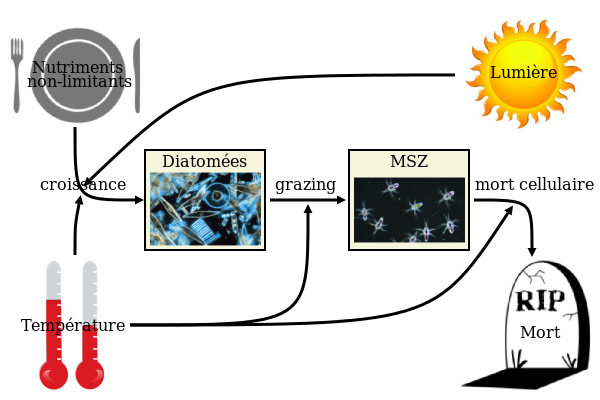
\includegraphics[width=\textwidth]{partie1/diagrammeConceptuel.png}
  \caption{Le modèle conceptuel du système étudié dans le quatrième cours. La croissance du phytoplancton
n'est plus limitée par les nutriments disponibles. Cependant, la croissance est toujours limitée par la
disponibilité de la lumière et de la température. Dans les formules, l'influence de ces deux impacts
environnementaux est cachée dans le terme $\mu_{DA}$. Une partie du phytoplancton existant est consommée
par le mésozooplancton (=MSZ). Cette partie est représentée par les différentes fonctions de broutage
fois la concentration du mésozooplancton ($graz_{MSZ}[MSZ]$). Dans le système modélisée
le mésozooplancton n'a pas des prédateurs naturels. Donc, la mort cellulaire naturelle du zooplancton ne peut
plus être négligée (dans les formules c'est le terme $mm_{MSZ}$ qui décrit cette l'influence).
}
  \label{fig:partie1DiagConcept}
\end{figure}

\par{
Pour peut mieux comprendre les équations du modèle, la grille~\ref{tab:partie1signifParam} peut également
être intéressante. Elle donne un aperçu de la signification etc. de chaque terme dans les équations.
}
\par{
Nous voulons encore pointer que $T_{opt}$ et $d_{opt}$ ont les mêmes valeurs pour les diatomées et le
mésozooplancton simulés. On a donc consideré que les deux espèces sont limitées par la tempèrature
de la même façon.
}

\begin{table}[h!]
\begin{center}
\begin{tabular}{ | c | c | c | c | c | }
\hline
Terme & Signification & Type & Valeur & Unité \\
\hline
$[DA]$ & \pbox{4cm}{Concentration du carbon des diatomées} & Variable d'état & $5$ & ${{mmol C}\over{m^{-3}}}$ \\
$[MSZ]$ & \pbox{4cm}{Concentration du carbon du mésozooplancton}  & Variable d'état & $1$ & ${{mmol C}\over{m^{-3}}}$ \\
$\mu_{DA}$ & \pbox{4cm}{Taux de croissance des diatomées} & \pbox{3cm}{Fonction $\mu_{max}max(T)llum$} & \pbox{4cm}{Dépend de la disponibilité de la lumière (en fonction du $[DA]$) et de la température} & $Jour^{-1}$ \\
$graz_{MSZ}$ & \pbox{4cm}{Fonction de grazing} & Fonction & \pbox{4cm}{Dépend de la température et de $[DA]$} & $Jour^{-1}$ \\
$eges_{MSZ}$ & \pbox{4cm}{Taux d'egestion du mésozooplancton} & Paramètre & $0.1$ & $-$ \\
$Y_{MSZ}$ & \pbox{4cm}{Efficience de croissance du mésozooplancton} & Paramètre & $0.25$ & $-$ \\
$mm_{MSZ}$ & \pbox{4cm}{Taux de mortalité du mésozooplancton} & Paramètre & $0.05$ & $Jour^{-1}$ \\
$g_{MSZ}$ & \pbox{4cm}{Taux de grazing maximal} & Paramètre & $1.2$ & $Jour^{-1}$ \\
$max(T)$ & \pbox{4cm}{Fonction de la limitation de la tempèrature} & \pbox{3cm}{Fonction\\(bell-shaped)} & \pbox{4cm}{Dépend de $T, T_{opt}$ et $d_{opt}$} & $-$ \\
$kg_{MSZ}$ & \pbox{4cm}{Constante de grazing} & Paramètre & $10$ & ${{mmol C}\over{m^{-3}}}$ \\
$[DA_0]$ & \pbox{4cm}{Concentration minimale avant que le mésozooplancton commence à consummer les diatomées} & Paramètre & $5$ & ${{mmol C}\over{m^{-3}}}$ \\
$\mu_{max}$ & \pbox{4cm}{Taux de croissance maximal des diatomées} & Paramètre & $1.2$ & $Jour^{-1}$ \\
$T_{opt}$ & \pbox{4cm}{Température optimale (pour les diatomées et le mésozooplancton)} & Paramètre & $16.3$ & $^{\circ}C$ \\
$d_{opt}$ & \pbox{4cm}{Delta T (pour les diatomées et le mésozooplancton)} & Paramètre & $13.7$ & $^{\circ}C$ \\
$T$ & \pbox{4cm}{Température simulée} & Paramètre & $10.0$ & $^{\circ}C$ \\
$llum$ & \pbox{4cm}{Limitation par la lumière} & \pbox{3cm}{Fonction\\$1-e^{-\alpha PAR_Z / \mu_{max}}$} & \pbox{4cm}{Dépend de la lumière disponible, ...} & $-$ \\
\end{tabular}
\end{center}
\end{table}
\clearpage
\begin{table}[h!]
\begin{center}
\begin{tabular}{ | c | c | c | c | c | }
$\alpha$ & \pbox{4cm}{L'efficacité des chloroplastes des diatomées} & Paramètre & $0.02$ & ${mol^{-1}*m^2*sec}\over{quanta * jour}$ \\
$PAR_Z$ & \pbox{4cm}{Lumière disponible par mol chlorophylle} & \pbox{3cm}{Fonction\\$PAR_0*e^{-k_e*z}$} & \pbox{4cm}{Dépend de la latitude, les solides en suspension, ...} & ${mol*quanta}\over{m^2*sec}$ \\
$PAR_0$ & \pbox{4cm}{Lumière solaire incidente} & Paramètre & $23.0$ & ${quanta}\over{m^2*sec}$ \\
$k_e$ & \pbox{4cm}{Coefficient d'extinction verticale de la lumière} & \pbox{3cm}{Fonction\\$0.35+0.02{{1}\over{2}}[DA]$} & \pbox{4cm}{Dépend des solides en suspension, ...} & $^{mol}/_m$ \\
$z$ & \pbox{4cm}{Profondeur de l'habitat} & Paramètre & $1.0$ & $m$ \\
\hline
\end{tabular}
\end{center}
  \caption{Signification, type, valeur et unité de chaque terme/paramètre dans les
équations~\ref{eq:partie1DiffEq1},~\ref{eq:partie1DiffEq2},~\ref{eq:partie1GrazMic},~\ref{eq:partie1GrazMicSeul} et~\ref{eq:partie1GrazHol}.}
  \label{tab:partie1signifParam}
\end{table}
\FloatBarrier

\subsection{Analyse mathématique}

\par{
La grille~\ref{tab:partie1etatsStat} donne un aperçu des états stationnaires du système
pour les diffèrentes fonctions de broutage. Les constantes supplémentaires utilisées
dans la grille sont définies comme suit:
}
\[
m = mm_{MSZ_{MAX_0}} e ^{- \left ( {{t-t_{opt}}\over{d_{opt}}} \right )}
\]
\[
k = kg_{MSZ}
\]
\[
c = \left ( 1 - eges_{MSZ} \right ) y_{MSZ}
g_{MSZ_{MAX_0}} e ^{- \left ( {{t-t_{opt}}\over{d_{opt}}} \right )}
\]
\[
f = g_{MSZ_{MAX_0}} e ^{- \left ( {{t-t_{opt}}\over{d_{opt}}} \right )}
\]

\begin{table}[h!]
\begin{center}
\begin{tabular}{ | c | c c | }
\hline
fct. de broutage & $[DA]$ & $[MSZ]$ \\
\hline
MIC, MIC\_Seul, HOL & 0 & 0 \\
MIC & $k * {{m}\over{c-m}}$ & ${{\mu_{DA} k \left ( 1 + {{m}\over{c-m}} \right )}\over{f}}$ \\
MIC\_Seuil & ${{m/c*k-m/c[DA_0]+[DA_0]}\over{1-m/c}}$ & ${\mu_{DA} * [DA] * (k + [DA] - [DA_0])}\over{f *([DA] - [DA_0])}$ \\
HOL & $k*\sqrt{{{m}\over{c-m}}}$ & ${{\mu_{DA}k \left ( 1 + {m}\over{c-m} \right )}\over{f \sqrt{{m}\over{c-m}}}}$ \\
\hline
\end{tabular}
\end{center}
  \caption{Les états stationnaires du système pour les diffèrentes fonctions de broutage. Les
constantes supplémentaires utilisées ont été définies dans le texte précédent. Les formules sont en accord
avec les simulations informatiques décrites ci-dessous (cmp. grille~\ref{tab:partie1appPropFctGrazing} et
figure~\ref{fig:partie1RefSimulations}).
}
  \label{tab:partie1etatsStat}
\end{table}
\FloatBarrier

\par{
Pas tous les états stationnaires listés dans le tableau~\ref{tab:partie1etatsStat} sont stables. Pour
étudier la stabilité des différents états stationnaires on doit établir la matrice jacobienne.
Malheureusement il nous a manque un peu de temps pour étudier la stabilité en détail.
}

\subsection{Comparaison des différents fonctions de grazing}

\par{
Dans une première étape l'aissez nous discuter l'impact de la fonction de grazing. La courbe des
diffèrentes trois fonctions a été tracée dans la figure~\ref{fig:partie1grazingFcts}.
On peut observer les propriétés suivantes:
}
\begin{itemize}
  \item Toutes les courbes sont en augmentation monotone et s'approchent à un taux croissance de valeur
$g_{MSZ} max(T)$. La dérivée seconde des équations~\ref{eq:partie1GrazMic} et~\ref{eq:partie1GrazMicSeul}
est strictement négative. En conséquence les courbes sont courbées vers la gauche. Au contraire, la
dérivée seconde de l'équation~\ref{eq:partie1GrazHol} est positive entre $[0, kg_{MSZ}]$
et négative dans la région $[kg_{MSZ}, \infty[$. Alors, pour toutes les valeurs dans la zone $[-kg_{MSZ},kg_{MSZ}]$
la courbe est courbée vers la gauche. En dehors de cette région la courbe est courbée vers la droite.
  \item Quand on est à des concentrations de diatomées faibles, l'équation~\ref{eq:partie1GrazMic}
donne le taux de croissance le plus élevé. Lorsque la concentration des diatomées dépasse $kg_{MSZ}$,
l'équation~\ref{eq:partie1GrazHol} donne le taux de croissance le plus élevé.
  \item La courbe de l'équation~\ref{eq:partie1GrazMicSeul} est déplacée par rapport à la
courbe de l'équation~\ref{eq:partie1GrazMic} sur l'axe des abscisses par $[DA_0]$. Par conséquent,
les courbes de l'équation~\ref{eq:partie1GrazMic} et de l'équation~\ref{eq:partie1GrazMicSeul}
se croisent seulement à l'infini.
  \item Les courbes des équations~\ref{eq:partie1GrazMicSeul} et~\ref{eq:partie1GrazHol}
ne se croisent pas dans la région $[0, \infty[$ quand $[DA_0]$ est supérieur à $0.25$.
(Point(s) d'intersection: $x = {^1/_2} \left ( 1 \pm \sqrt{1 - 4 [DA_0]}\right )$).
\end{itemize}

\begin{figure}[h!]
  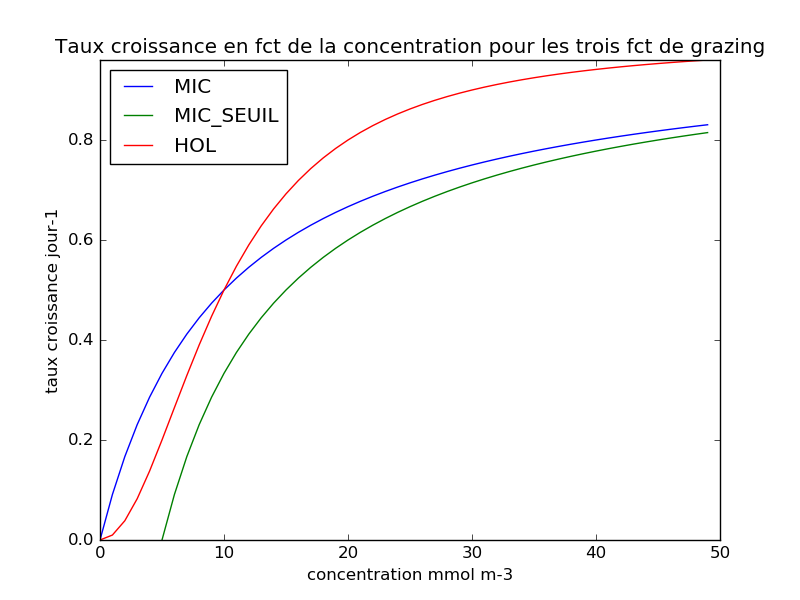
\includegraphics[width=\textwidth]{partie1/grazingFct.png}
  \caption{
La courbe des trois fonctions~\ref{eq:partie1GrazMic} (MIC),~\ref{eq:partie1GrazMicSeul} (MIC\_SEUIL)
et~\ref{eq:partie1GrazHol} (HOL) en fonction de la concentration $[DA]$.
}
  \label{fig:partie1grazingFcts}
\end{figure}

\par{
En utilisant ces propriétés, nous pouvons maintenant discuter de certaines simulations (voir
figure~\ref{fig:partie1RefSimulations}) pour mieux étudier l'impact de la fonction de grazing.
Le tableau~\ref{tab:partie1appPropFctGrazing} donne une vue synoptique sur les maximas et l'état
stationnaire du modèle pour les fonctions de grazing étudiées.
}
\begin{table}[h!]
\begin{center}
\begin{tabular}{ | c | c c | c c | c c |}
\hline
Fonction & \multicolumn{2}{c|}{Maximum $[DA]$} & \multicolumn{2}{c|}{Maximum $[MSZ]$} &
\multicolumn{2}{c|}{État stat.} \\
de grazing & Temps & Conc. & Temps & Conc. & $[DA]$ & $[MSZ]$ \\
\hline
MIC (voir eq.~\ref{eq:partie1GrazMic}) & $21.84$ & $87.474$ & $30.36$ & $39.992$ & $0.0$ & $0.0$ \\
MIC\_SEUIL (voir eq.~\ref{eq:partie1GrazMicSeul}) & $22.86$ & $112.107$ & $32.04$ & $45.979$ & $7.273$ & $10.478$ \\
HOL (voir eq.~\ref{eq:partie1GrazHol}) & $18.42$ & $60.979$ & $25.44$ & $29.276$ & $4.767$ & $7.016$ \\
\hline
\end{tabular}
\end{center}
  \caption{Les simulations (cmp. figure~\ref{fig:partie1RefSimulations}) montrent des maximas et
des états stationnaires différents. Ce tableau donne une vue synoptique sur les maximas
(temps et concentration) et l'état stationnaire du modèle pour les différentes fonctions de grazing
(cmp. fonctions~\ref{eq:partie1GrazMic},~\ref{eq:partie1GrazMicSeul} et~\ref{eq:partie1GrazHol}).}
  \label{tab:partie1appPropFctGrazing}
\end{table}

\par{
Au début des simulations, la concentration des diatomées et du mésozooplancton augmentent de
façon exponentielle. Les diatomées peuvent assurer cette croissance rapide parce que la concentration du
mésozooplancton et des diatomées est relativement petite. Du coup le terme $graz_{MSZ} [MSZ]$ est
``insignifiant'' en comparaison avec le terme $\mu_{DA}[DA]$. On peut quand même observer certaines
différences dans la pente des courbes. Ces différences se basent sur les différentes fonctions de grazing
utilisées. L'équation de Michaelis-Menton (equation~\ref{eq:partie1GrazMic}) montre (en comparaison avec
les autres équations) les valeurs les plus grandes pour les concentrations des diatomées faibles.
On conséquence, dans cette simulation la pente de la courbe des diatomées commence à augmenter plus lentement
que dans les autres simulations. Une fois la concentration de $[DA]$ est plus grande que $kg_{MSZ}$,
c'est la fonction de Holling (equation~\ref{eq:partie1GrazHol}) qui limite le plus. Donc à partir de
cette concentration c'est la fonction de Holling qui limite le plus.
}
\par{
Au fil du temps la concentration du mésozooplancton continue de croître. Le plus grands la valeur 
de cette concentration deviendra, les plus limitant devient l'impact de cette espèce sur la croissance
des diatomées (terme: $-graz_{MSZ}$). C'est pour ça que à partir d'un moment donné, la concentration
des diatomées commence à diminuer.
}
\par{
Peu de temps après la concentration du mésozooplancton commence à décliner égalèment, parce que
l'impacte du taux de mortalité devient plus grand que le terme de croissance $(1-eges_{MSZ})graz_{MSZ}Y_{MSZ}$.
(Il y manque des diatomées comme nuriture.) Les concentrations des diatomées et du mésozooplancton
commencent à converger vers l'état stationnaire. De manière générale le maxium de les diatomées est
toujours plus grands que cel du mésozooplancton.
}
\par{
Comme on peut voir dans le tableau~\ref{tab:partie1appPropFctGrazing}) on observe quand même des
grands différents dans la hauteure et le moment les maximums des concentrations deroullent
pour les fonctions de grazing diffèrente. (On voit égalément des valeurs differents pour l'état
stationnaire; cmp. tableau~\ref{tab:partie1etatsStat}.)
Dans les sous-chapitres souivants nous décortiquons explicitement ces différences en fonction de la
fonction de grazing.
}

\subsubsection{La fonction de Michaelis-Menton}
\par{
Dans le cas d'une fonction de type Michaelis-Menton (équation~\ref{eq:partie1GrazMic}) on observe les
graphiques dans la première ligne dans la figure~\ref{fig:partie1RefSimulations}. On voit que
la biomasse des diatomées maximale et la biomasse du mésozooplancton maximale arrivent plus tard que
pour la fonction de Holling (equation~\ref{eq:partie1GrazHol}, cmp. dernière ligne dans la
figure~\ref{fig:partie1RefSimulations}). En plus les maximas sont plus élevées (voir
tableau~\ref{tab:partie1appPropFctGrazing}, cmp. figure~\ref{fig:partie1RefSimulations}).
En effet, la valeur du taux de grazing aux hautes concentrations est plus faible pour la fonction de
Michaelis-Menton (equation~\ref{eq:partie1GrazMic}) que pour la fonction de Holling
(equation~\ref{eq:partie1GrazHol}). Donc les diatomées peut croître de manière plus que dans le cas de
la fonction de Holling.
}
\par{
Cependant, la population des diatomées tombe à zéro à partir du 30ème jour. C'est parce que peu de
temps après on rencontré le maximum dans la biomasse des diatomées. Donc, on observe une situation ou
la concentration du mésozooplancton est grande, mais la concentration en diatomées est faible.
La fonction de Michaelis-Menton donne des valeurs relativement haute pour une population des diatomées
petite (en comparison avec les deux autres fonctions de grazing). L'impact de la fonction Michaelis-Menton
reste alors grand, ce qu'entraînant l'extinction des diatomées. Quand il y en a plus des diatomées,
le taux de grazing tombe aussi à zéro. Le seul terme restent c'est donc le terme de mortalité du
mésozooplancton. Donc la concentration du mésozooplancton diminuera aussi. (Jusque la biomasse du
mésozooplancton disparaisse.)
}
\subsubsection{La fonction de Michaelis-Menton avec seuil}
\par{
Dans le cas de l'équation de Michaelis-Menton avec seuil (voir équation~\ref{eq:partie1GrazMicSeul}),
la biomasse maximale des diatomées et du mésozooplancton arrivent encore plus tard et sont encore plus
élevées (cmp. deuxième ligne dans la figure~\ref{fig:partie1RefSimulations},
tableux~\ref{tab:partie1appPropFctGrazing}) que dans le cas de l'équation de Holling. De manière générale
(si $kg_{MSZ} < 0.25$), le taux de grazing
calcule en outilisent la fonction de Michaelis-Menton avec seuil est toujours plus faible que cels calculent
en outilisent les autres fonctions. La population des diatomées a alors plus de temps pour croître.
Du coup le maximum va être atteindre plus tard et sera plus élevée.
}
\par{
Comme dit, aussi pour des faible concentration des diatomées, le taux de grazing calcule en outilisent
la formule de Michaelis Menton avec seuil est plus faible que cel calcule en outilisent la fonction de
Holling. Donc l'équilibre se fait à des concentrations plus importantes.
Ici, comme le taux de croissance en fonction de la concentration possède une seuil ($[DA_0]$), l'équilibre
s'effectue autour de ce seuil, plus ou moins $[DA_0]$ (cmp. grille~\ref{tab:partie1etatsStat}).
}
\subsubsection{La fonction de Holling}
\par{
Dans le cas de l'équation de Holling (voir equation~\ref{eq:partie1GrazHol}) la croissance du
phytoplancton (le terme de croissance est supérieure au terme de mortalité) persiste de
$t=0$ à $t\approx 18$ jours (voir tableau~\ref{tab:partie1appPropFctGrazing}, cmp. dernière ligne
dans la figure~\ref{fig:partie1RefSimulations}). Le valeur maximal vaut $\approx 60 {^mmol}/_{m^3}$ 
(cmp. tableau~\ref{tab:partie1appPropFctGrazing}). Après ce maximum était obtenu la concentration 
du phytoplancton diminue car le terme de mortalité est supérieure du terme de croissance.
}
\par{
Ce développement continue, jusqu'on atteind un minimum de $\approx 3 {^mmol}/_{m^3}$
des diatomées au 28ème jour. Par la suite, la concentration reaugment jusque la
concentration des diatomées et du mésozooplancton se stabilisées au état
stationnaire (cmp. grille~\ref{tab:partie1etatsStat}).
}

\begin{figure}[h]
  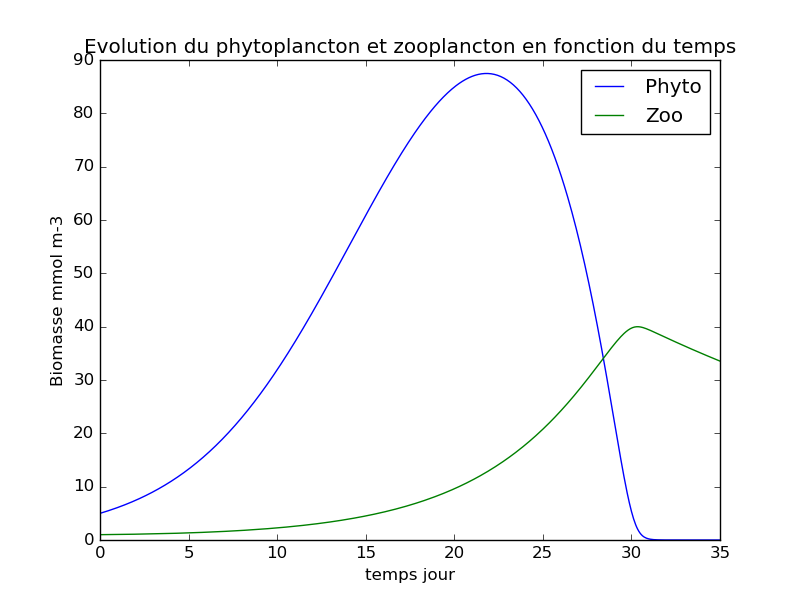
\includegraphics[width=0.5\textwidth]{partie1/refMic35.png}\hfill
  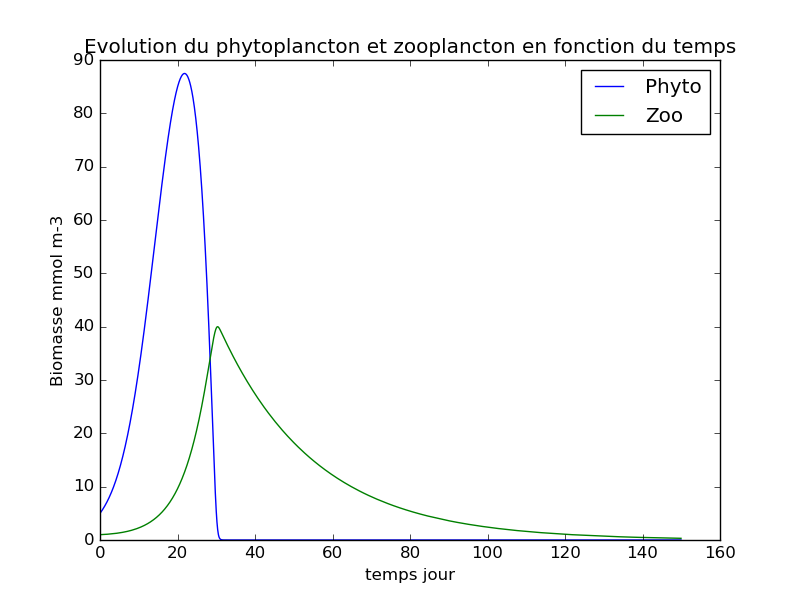
\includegraphics[width=0.5\textwidth]{partie1/refMic150.png}\\
  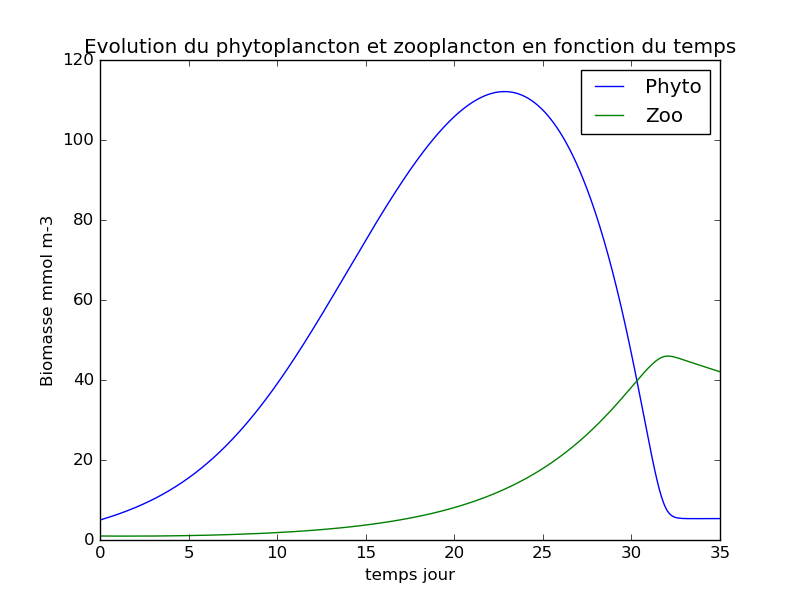
\includegraphics[width=0.5\textwidth]{partie1/refMicSeul35.png}\hfill
  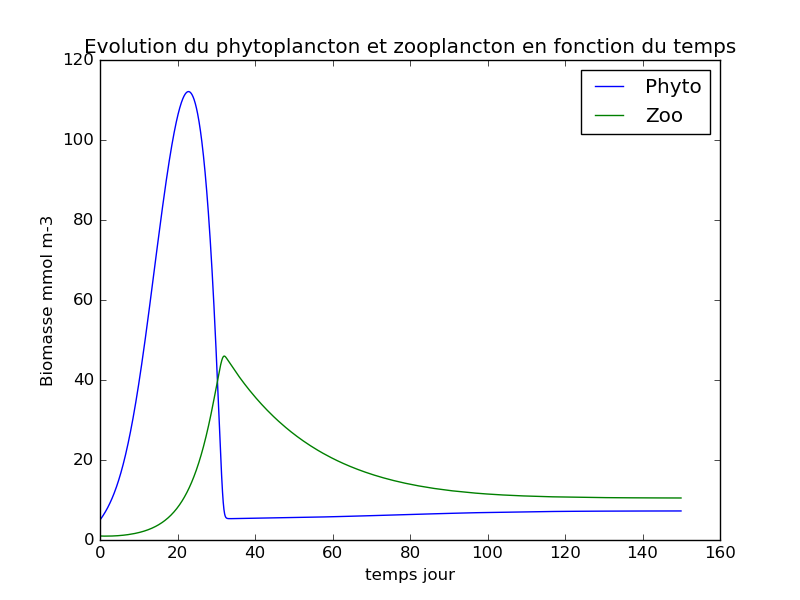
\includegraphics[width=0.5\textwidth]{partie1/refMicSeul150.png}\\
  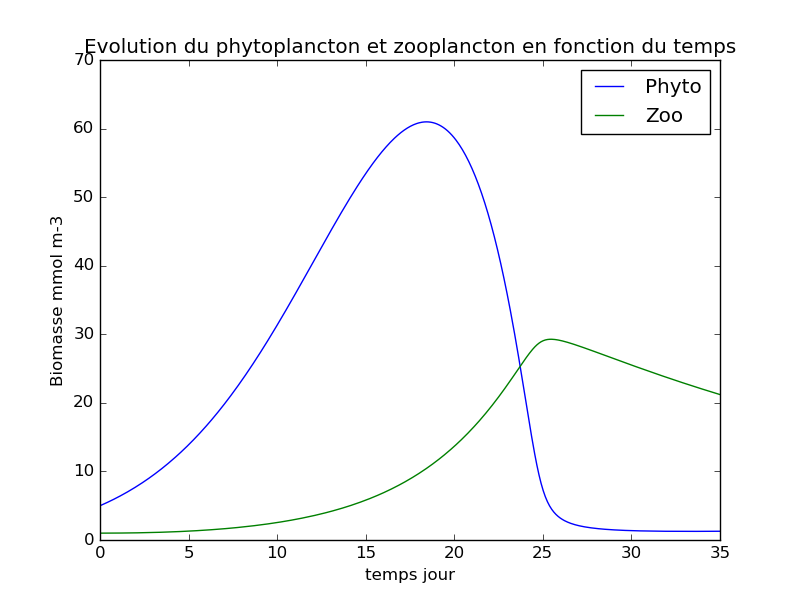
\includegraphics[width=0.5\textwidth]{partie1/refHol35.png}\hfill
  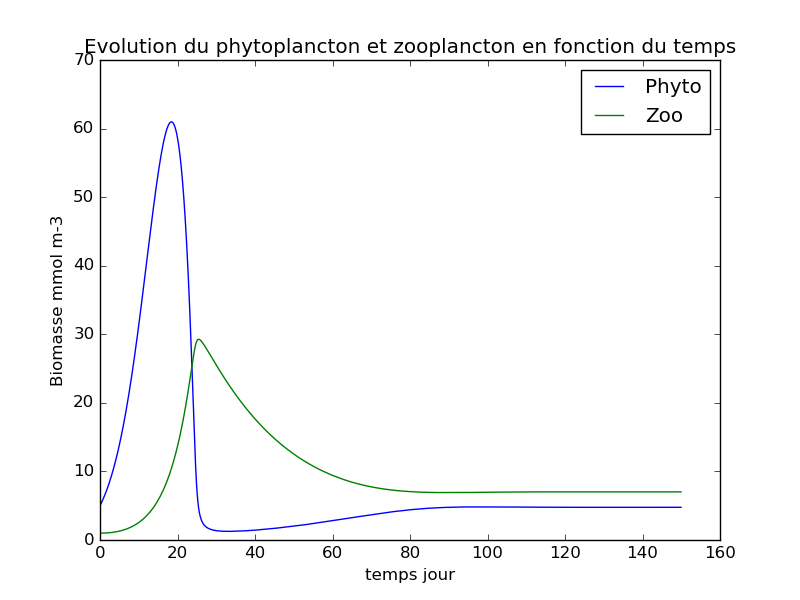
\includegraphics[width=0.5\textwidth]{partie1/refHol150.png}
  \caption{Les simulations de références pour les fonctions diffèrente de grazing (
fonction de Michaelis-Menton (eq.~\ref{eq:partie1GrazMic}, première ligne),
Michaelis-Menton avec seuil (eq.~\ref{eq:partie1GrazMicSeul}, deuxième ligne) et fonction de
Holling (eq.~\ref{eq:partie1GrazHol}, ligne terminale)) pour des temps final diffèrente.
Avec un temps final de 35 jours la colonne de gauche montre une sous-partie des graphiques
de la colonne de droite. La colonne de droite montre le cours de simulation jusqu'à un temps
final de 150 jours.}
  \label{fig:partie1RefSimulations}
\end{figure}

\clearpage
\subsection{Changements des paramètres}

\par{
Dans une deuxième étappe on a aussi modifier quelques paramètres pour explorer leur impact sur le system.
}

\subsubsection{Test 1 - Augmentation du taux de grazing maximal}
\begin{figure}[h!]
  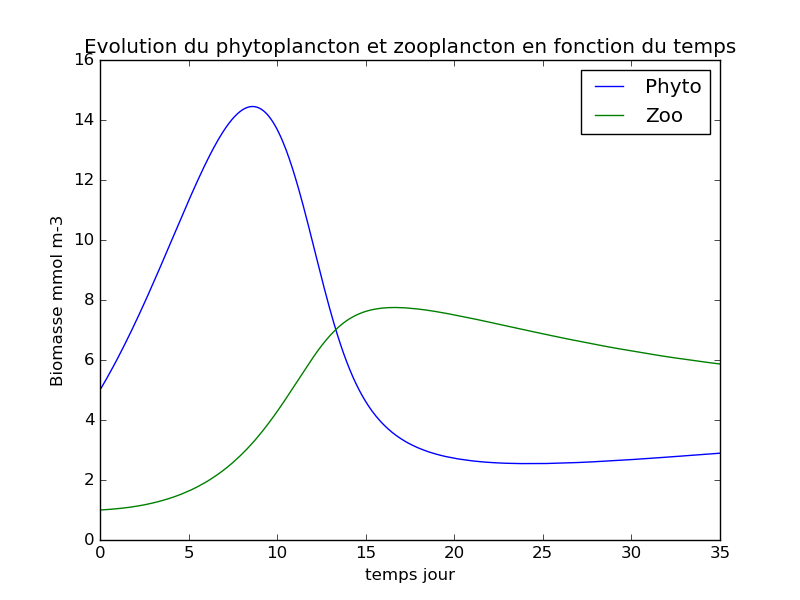
\includegraphics[width=\textwidth]{partie1/test1x35.png}
  \caption{Simulation de l'impact de l'augmontation du taux de grazing maximal. Pour cette simulation,
on a augmonté la constante $g_{MSZ_{max0}}$ de $1.2$ à $2$ par rapport à la simulation de référence.}
  \label{fig:partie1t1}
\end{figure}
\par{
Comme on peut voir dans la figure~\ref{fig:partie1t1}, quand on augmonte le taux de grazing maximal, 
les maximas sont atteint plus rapidement, et atteignent une valeur plus faible pour les deux population.
En effet, le taux de grazing a augmenté, et donc, le terme croissance des diatomées devient plus rapidement
égal à la mortalité. De la même manière, le mésozooplancton croisse moins que dans la simulation de référence,
puisque la concentration des diatomées est plus faible.
}
\subsubsection{Test 2 - Augmentation du taux de demi-saturation du mésozooplancton}
\begin{figure}[h!]
  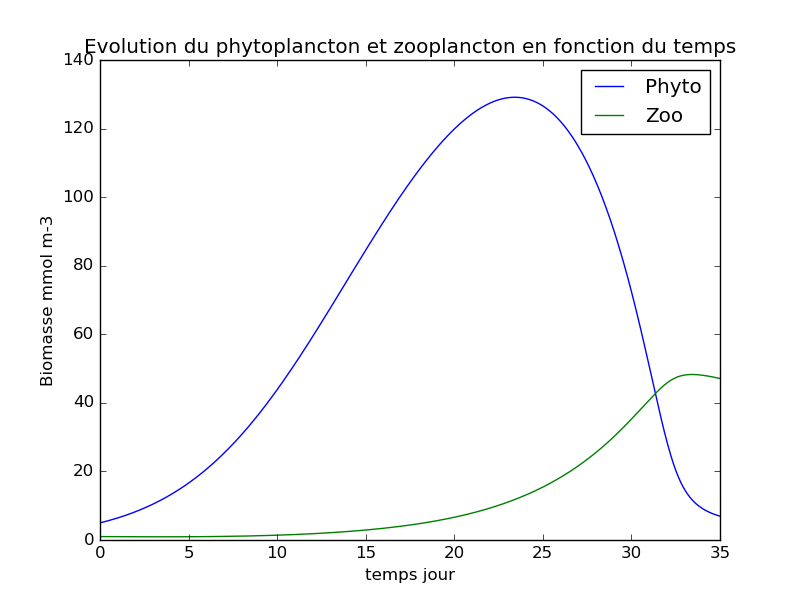
\includegraphics[width=\textwidth]{partie1/test2x35.png}
  \caption{Simulation de l'impact de l'augmontation du taux du demi-saturation du mésozooplancton. Pour
cette simulation, on a augmonté la constante $kg_{MSZ}$ de $10$ à $25$ par rapport à la simulation de
référence.}
  \label{fig:partie1t2}
\end{figure}
\par{
Quand on augmonte le taux de demi-saturation du mésozooplancton (voir figure~\ref{fig:partie1t2})
on entraine une diminution de l'affinité du mésozooplancton pour les diatomées. Ainsi, les diatomées
atteignent leur maximum plus tard, et le maximum est plus important. Ceci permet une croissance plus
importante pour le mésozooplancton. Donc le maxium du mésozooplancton est atteint plus tard,
et a une valeur plus grande. 
}
\FloatBarrier

\clearpage
\subsubsection{Test 3 - Dimination du taux de demi-saturation du mésozooplancton}
\begin{figure}[h!]
  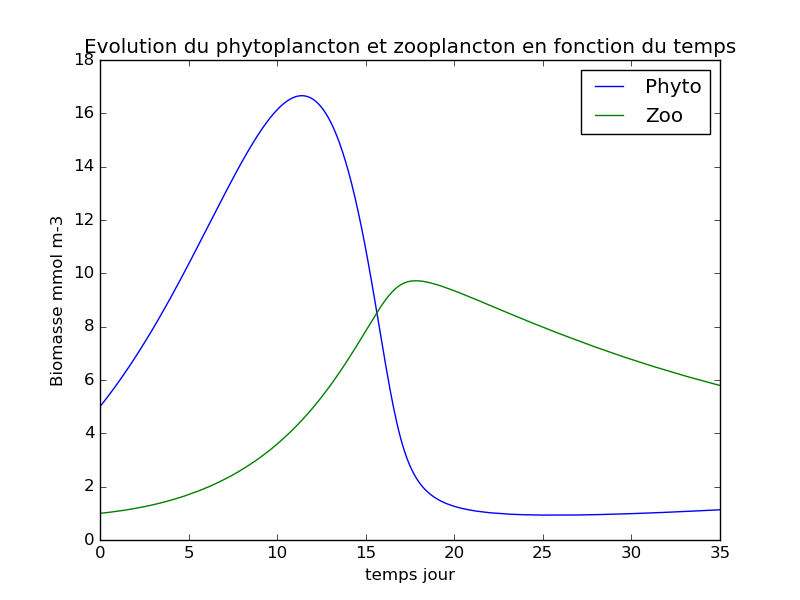
\includegraphics[width=\textwidth]{partie1/test3x35.png}
  \caption{Simulation de l'impact de la dimination du taux du demi-saturation du mésozooplancton. Pour
cette simulation, on a diminué la constante $kg_{MSZ}$ de $10$ à $5$ par rapport à la simulation de
référence.}
  \label{fig:partie1t3}
\end{figure}
\par{
Quand on diminue le taux de demi-saturation du mésozooplancton (voir figure~\ref{fig:partie1t3}) on observe
l'inverse que dans la simulation précédente. On augmentate l'affinité du mésozooplancton pour les diatomées,
car le taux de grazing devient plus grand pour les même concentrations. Ainsi, les diatomées ont un maximum plus
faible qui arrive plus vite. En conséquence le maximum du mésozooplancton va aussi arriver plus vite (et sera
moins élevé).
}
\FloatBarrier

\clearpage
\subsubsection{Test 4 - Augmentation de l'efficacité de grazing}
\begin{figure}[h!]
  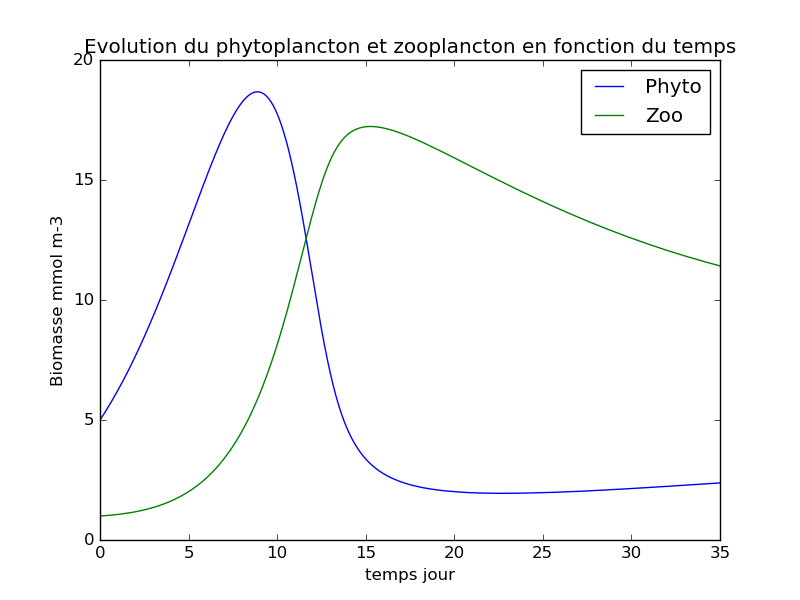
\includegraphics[width=\textwidth]{partie1/test4x35.png}
  \caption{Simulation de l'impact de l'augmontation de l'efficacité de grazing du mésozooplancton. Pour
cette simulation, on a augmonté la constante $Y_{MSZ}$ de $0.25$ à $0.5$ par rapport à la simulation de
référence.}
  \label{fig:partie1t4}
\end{figure}
\par{
Dans le cinquième test on a augmonte l'efficacité de grazing (graphique simulée, voir
figure~\ref{fig:partie1t4}).
La concentration maximale des diatomées est atteinte plus rapidement (et elle est plus faible), car
le mésozooplancton consomme plus efficacement les diatomées que dans la simulation de référence. Du coup le 
le terme de mortalité dans l'equation~\ref{eq:partie1DiffEq1} compense plus rapidement le terme de
croissance. Ainsi, pour une même concentration des diatomées, on arrivra à une concentration de
mèsozooplancton plus grande (le terme de croissance pour le mésozooplancton peut devenir plus facilement plus
grand).
}
\FloatBarrier

\clearpage
\subsubsection{Test 5 - Diminution du taux de la mortalité du mésozooplancton}
\begin{figure}[h!]
  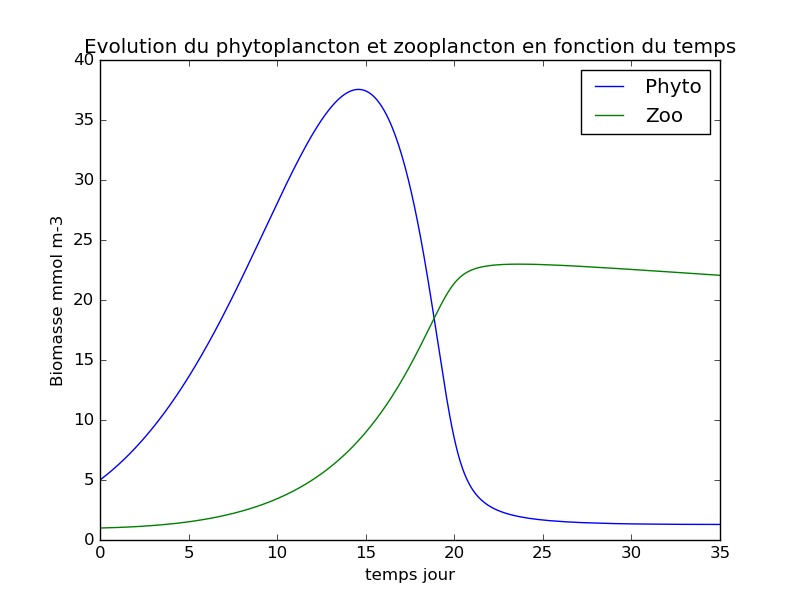
\includegraphics[width=\textwidth]{partie1/test5x35.png}
  \caption{Simulation de l'impact de la dimination du taux de la mortalité du mésozooplancton. Pour
cette simulation, on a diminué la constante $mm_{MSZ}$ de $0.05$ à $0.01$ par rapport à la simulation de
référence.}
  \label{fig:partie1t5}
\end{figure}
\par{
Ici on a diminué le taux de la mortalité du mésozooplancton (voir figure~\ref{fig:partie1t5}).
Pour un taux de mortalité plus faible, la concentration de mésozooplancton diminura moins rapidement que
dans la simulation de référence. De plus, puisque le taux de mortalité est faible, on observe des
concentrations du mésozooplancton plus élvées. De façon inverse, quand la concentration du mésozooplancton
est plus élvée, les diatomées pouvent croître moins facillement. Donc la concentration des diatomées est
plus faible et le maximum est atteint plus rapidement.
}
\FloatBarrier
